\begin{figure}
	\centering
	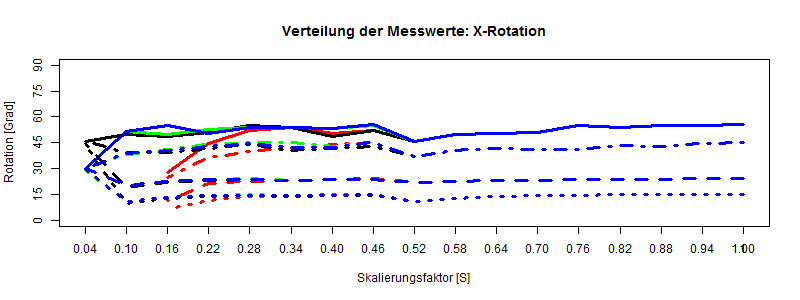
\includegraphics[width=\linewidth]{img_Skalierung/Skal_Max_RX}
	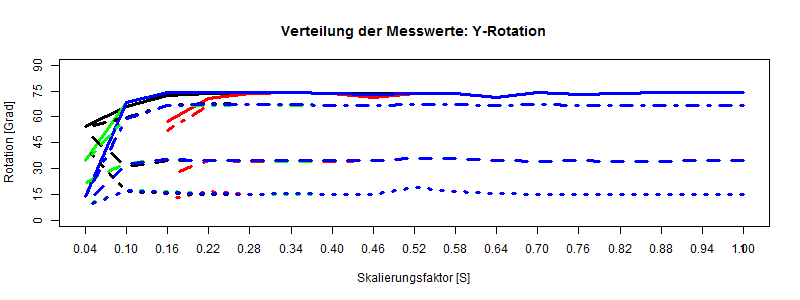
\includegraphics[width=\linewidth]{img_Skalierung/Skal_Max_RY}
	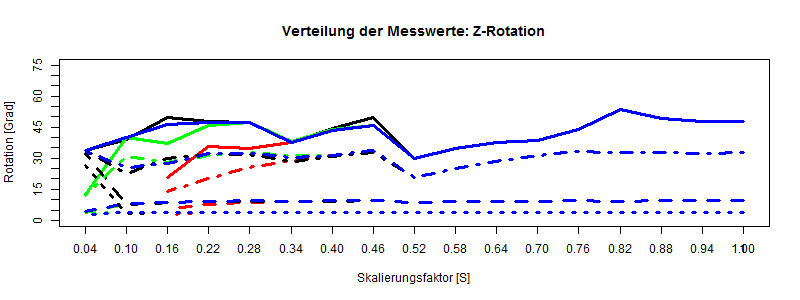
\includegraphics[width=\linewidth]{img_Skalierung/Skal_Max_RZ}
	\caption{Dargestellt ist der Bereich in denen im Biwi Kinect Head Pose Database \cite{BIWI_database} ein Gesicht erkannt wurde.\\
		Bicubic (blau), Lanczos (grün), Linear (schwarz), Nearest-Neighbor (rot)\\
		Maximal erreichter Wert: \protect
\includegraphics[width=0.15\linewidth]{line/Line1}\\
		$99,5\%$ Quantile der Messwerte: \protect
\includegraphics[width=0.15\linewidth]{line/Line4}\\
		$80\%$ Quantile der Messwerte:\protect
\includegraphics[width=0.15\linewidth]{line/Line2}\\
		Median aus den Messwerten: \protect
\includegraphics[width=0.15\linewidth]{line/Line3}}
	\label{img_Rot_Max}
\end{figure}
\begin{landscape}
\begin{figure}
	\centering
	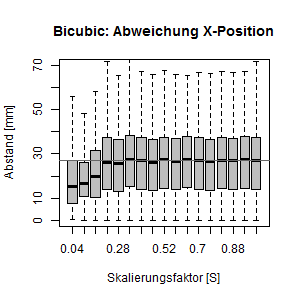
\includegraphics[width=0.245\linewidth]{img_Skalierung/CU_Tx}
	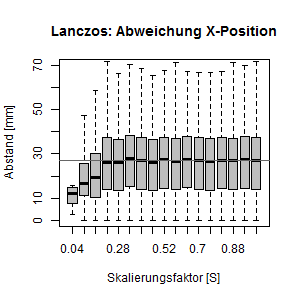
\includegraphics[width=0.245\linewidth]{img_Skalierung/LA_Tx}
	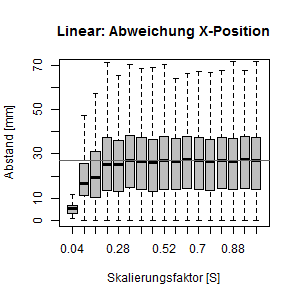
\includegraphics[width=0.245\linewidth]{img_Skalierung/LI_Tx}
	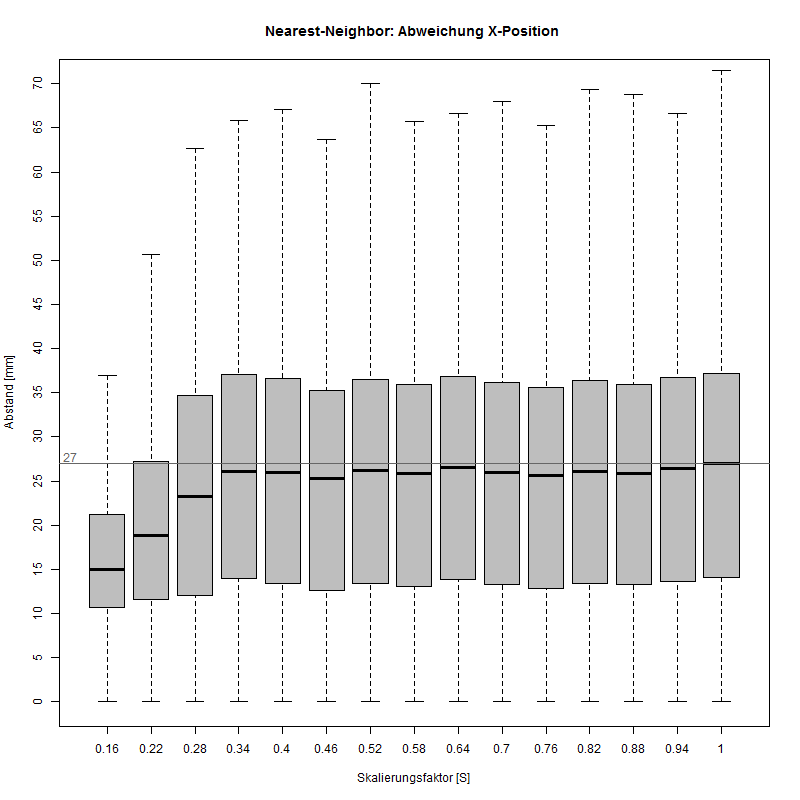
\includegraphics[width=0.245\linewidth]{img_Skalierung/NN_Tx}
	\caption{Zusammenhang zwischen der Skalierung und der Abweichung in X-Richtung in Millimeter.\\
		Von rechts nach links: Bicubic, Lanczos, Linear, Nearest-Neighbor}
	\label{img_X_Pos_Skal}
\end{figure}
\begin{figure}
	\centering
	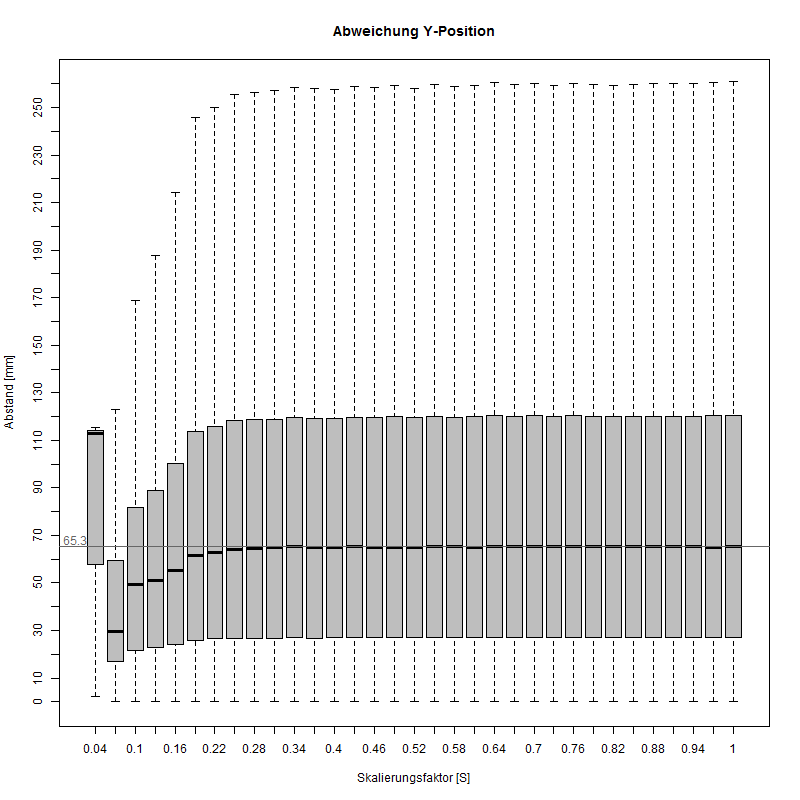
\includegraphics[width=0.245\linewidth]{img_Skalierung/CU_Ty}
	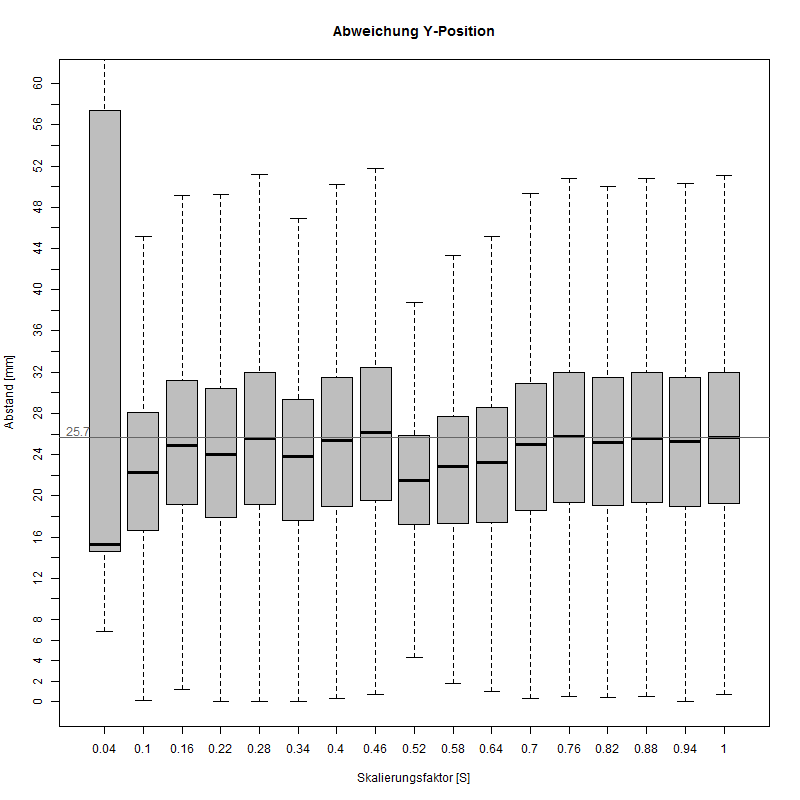
\includegraphics[width=0.245\linewidth]{img_Skalierung/LA_Ty}
	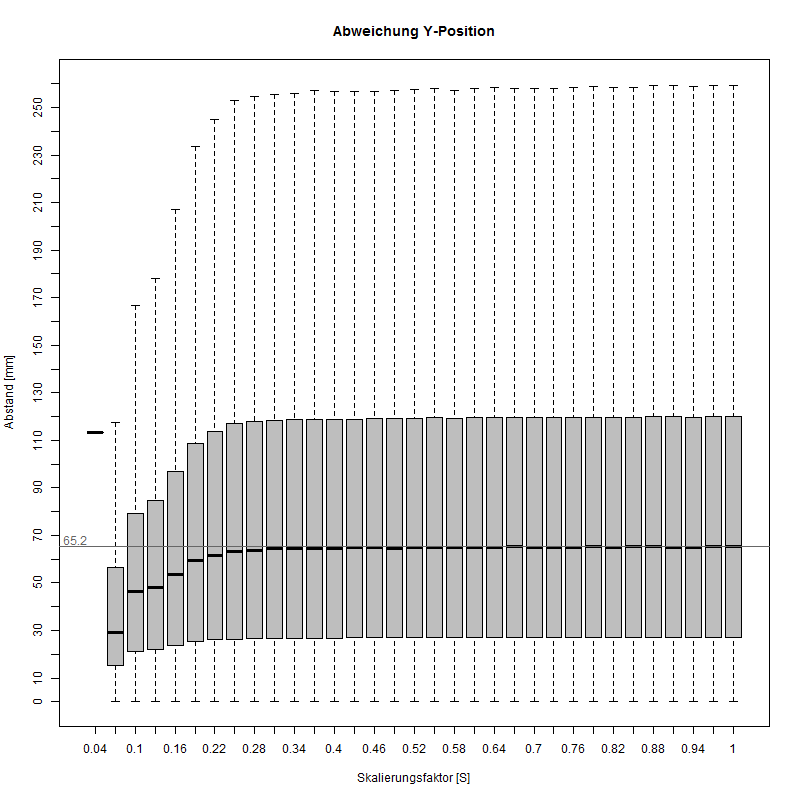
\includegraphics[width=0.245\linewidth]{img_Skalierung/LI_Ty}
	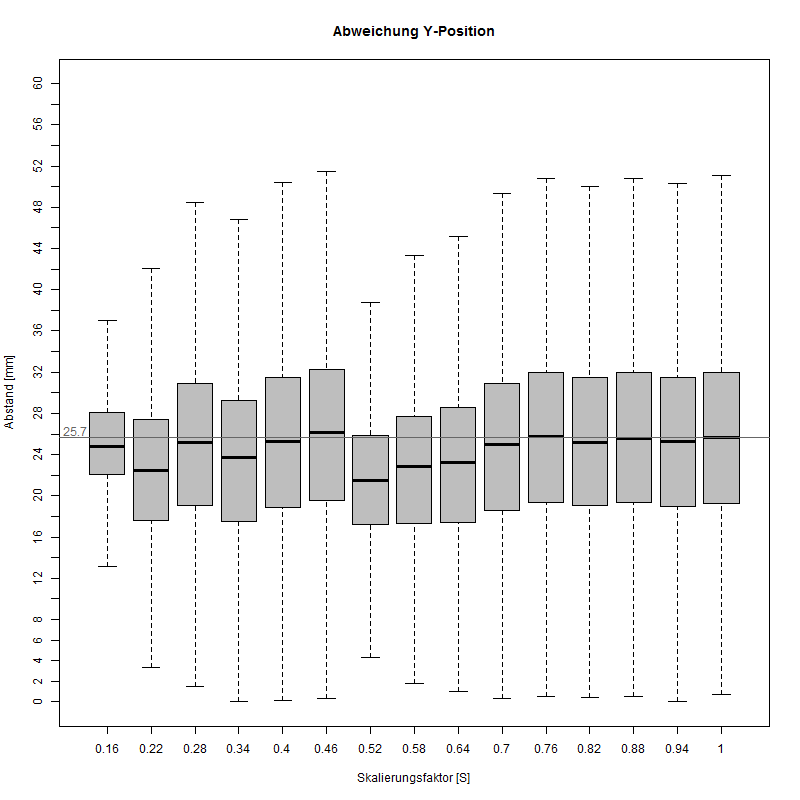
\includegraphics[width=0.245\linewidth]{img_Skalierung/NN_Ty}
	\caption{Zusammenhang zwischen der Skalierung und der Abweichung in Y-Richtung in Millimeter.\\
		Von rechts nach links: Bicubic, Lanczos, Linear, Nearest-Neighbor}
	\label{img_Y_Pos_Skal}
\end{figure}
\begin{figure}
	\centering
	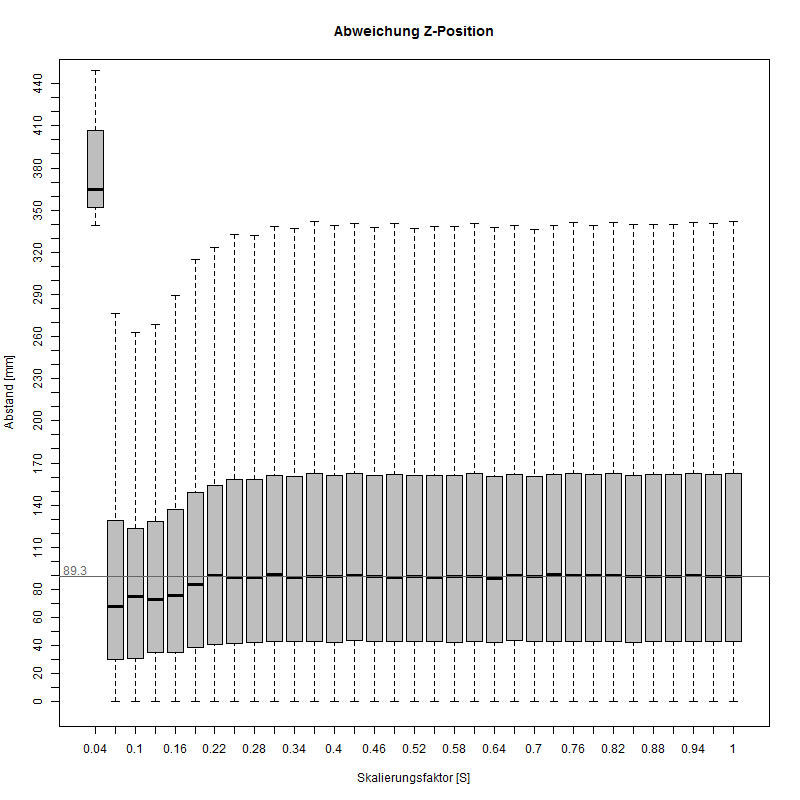
\includegraphics[width=0.245\linewidth]{img_Skalierung/CU_Tz}
	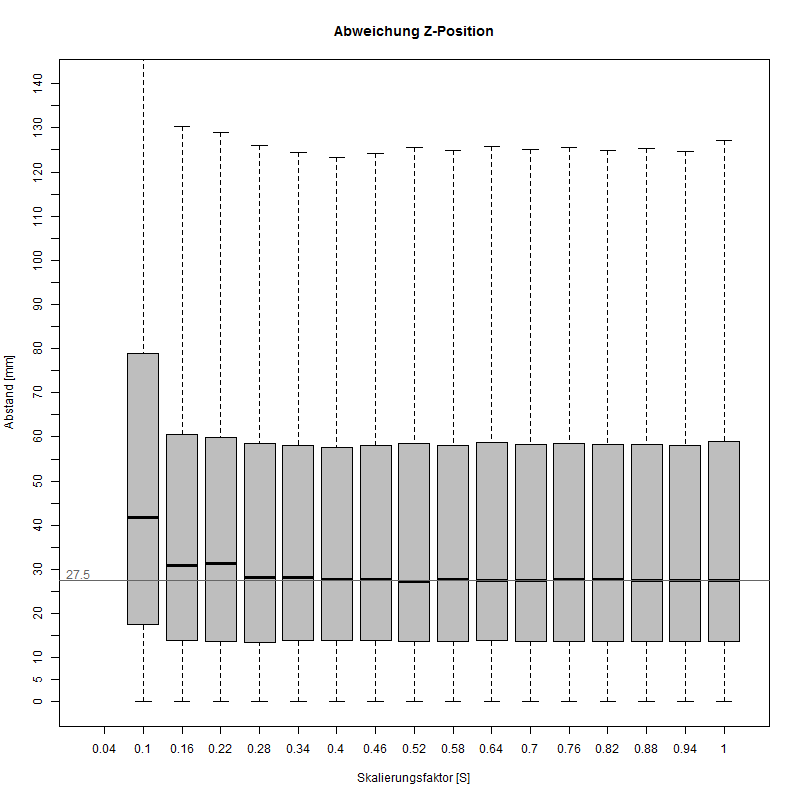
\includegraphics[width=0.245\linewidth]{img_Skalierung/LA_Tz}
	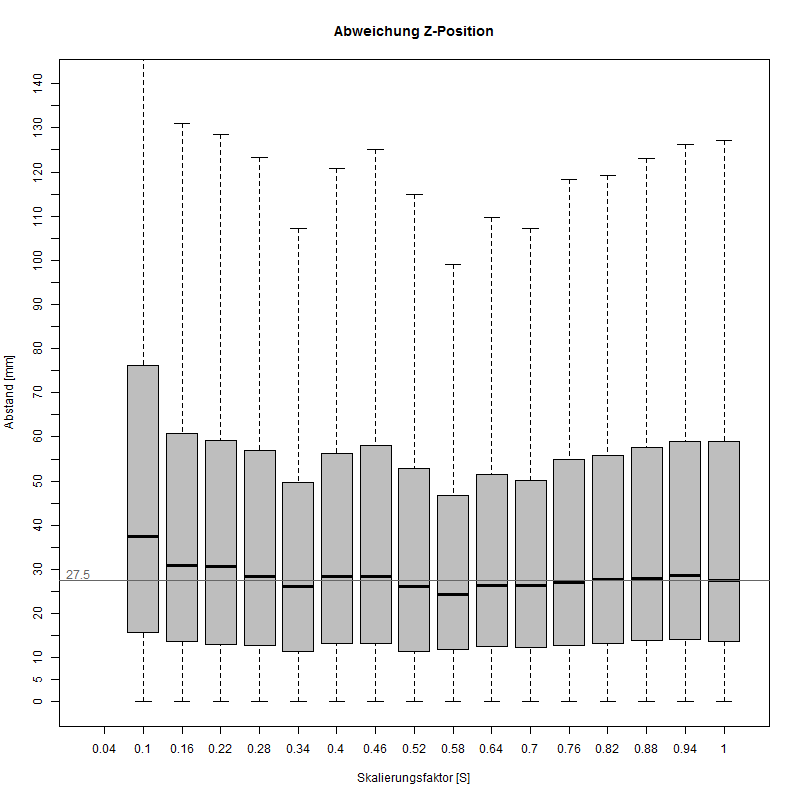
\includegraphics[width=0.245\linewidth]{img_Skalierung/LI_Tz}
	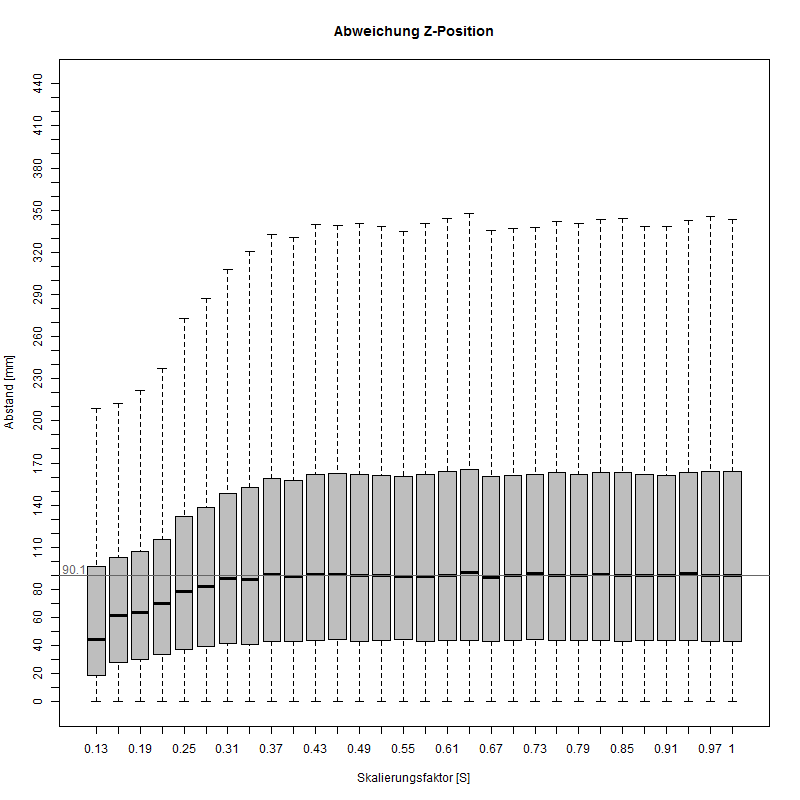
\includegraphics[width=0.245\linewidth]{img_Skalierung/NN_Tz}
	\caption{Zusammenhang zwischen der Skalierung und der Abweichung in Z-Richtung in Millimeter.\\
		Von rechts nach links: Bicubic, Lanczos, Linear, Nearest-Neighbor}
	\label{img_Z_Pos_Skal}
\end{figure}
%-----------------------------------------------------
\begin{figure}
	\centering
	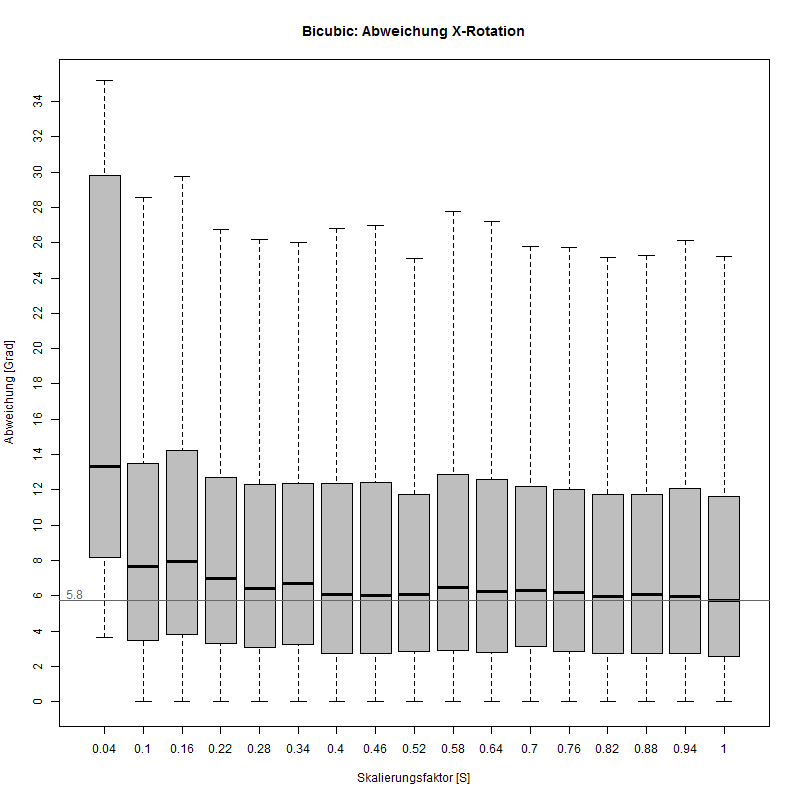
\includegraphics[width=0.245\linewidth]{img_Skalierung/CU_Rx}
	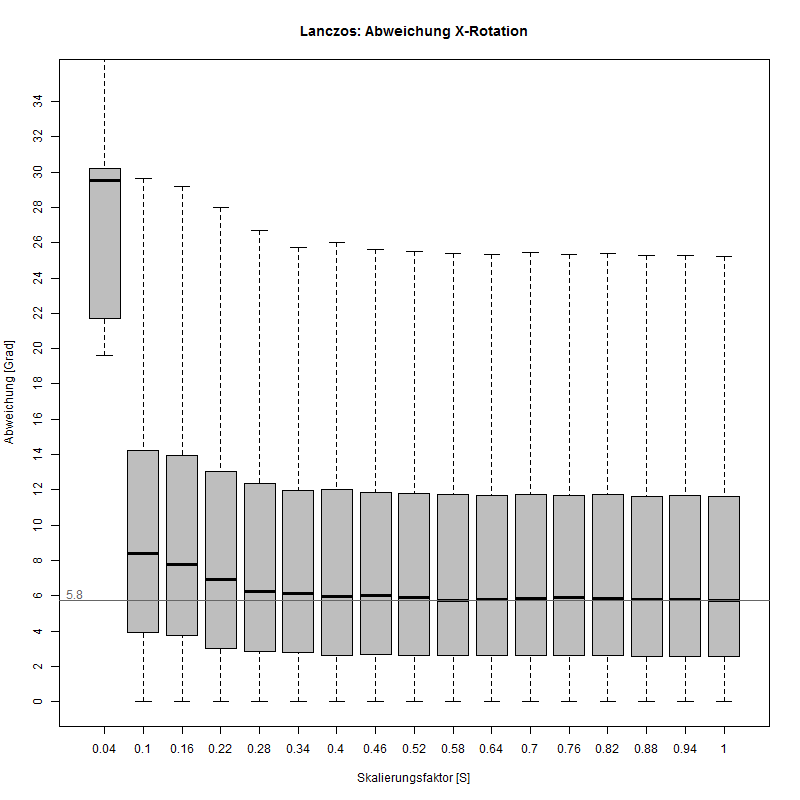
\includegraphics[width=0.245\linewidth]{img_Skalierung/LA_Rx}
	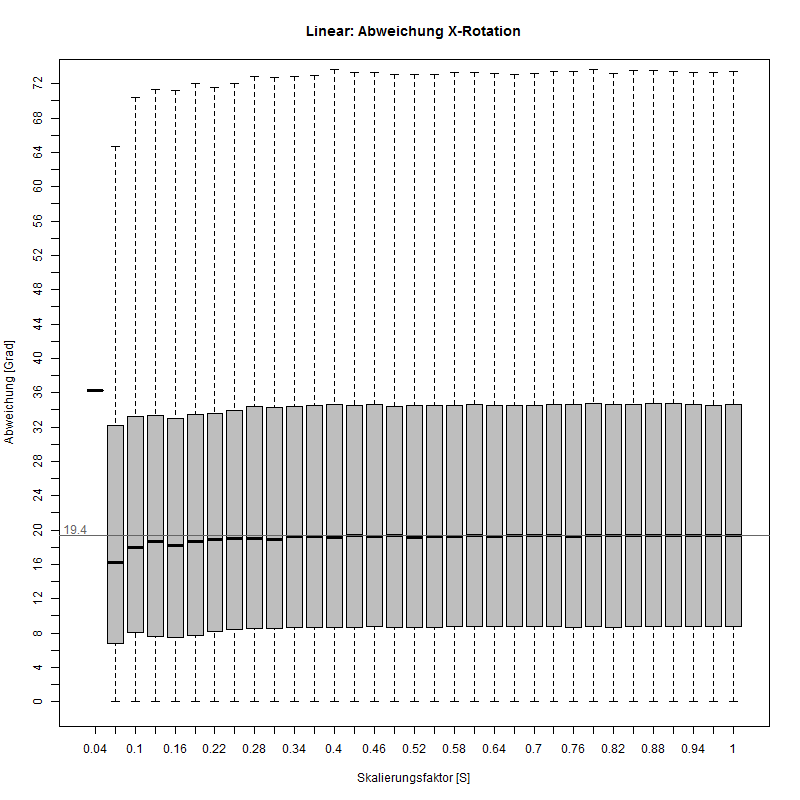
\includegraphics[width=0.245\linewidth]{img_Skalierung/LI_Rx}
	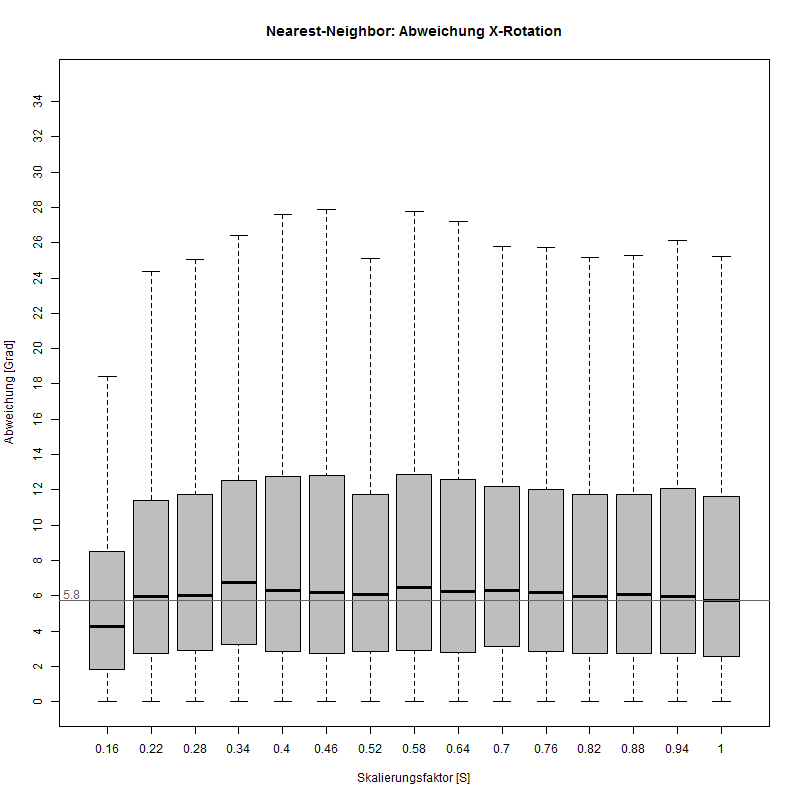
\includegraphics[width=0.245\linewidth]{img_Skalierung/NN_Rx}
	\caption{Zusammenhang zwischen der Skalierung und der Abweichung des Winkels in X-Richtung, Angabe in Bogenmaß.\\
		Von rechts nach links: Bicubic, Lanczos, Linear, Nearest-Neighbor}
	\label{img_X_Rot_Skal}
\end{figure}
\begin{figure}
	\centering
	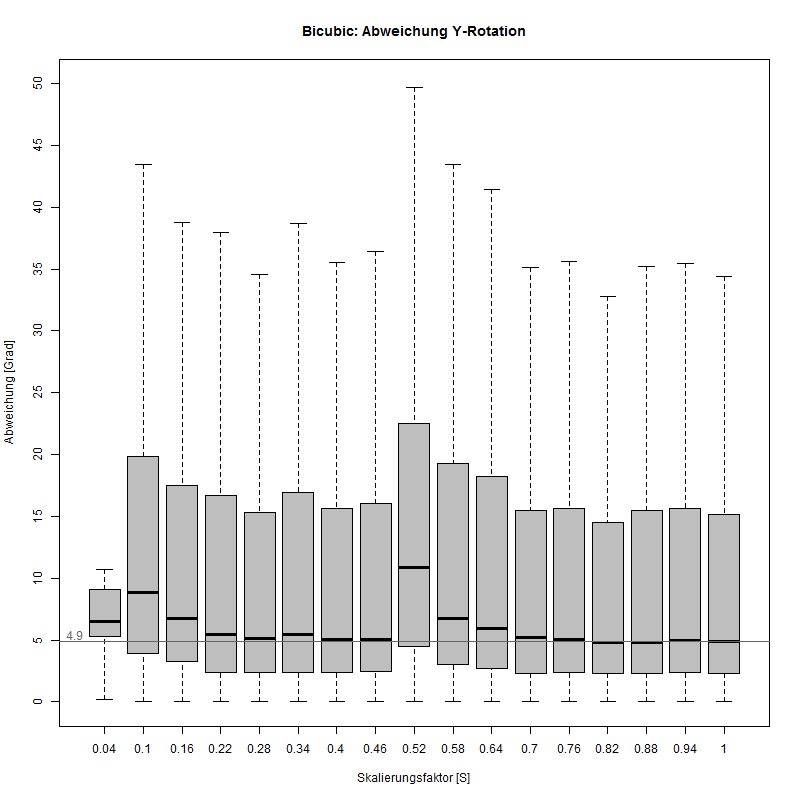
\includegraphics[width=0.245\linewidth]{img_Skalierung/CU_Ry}
	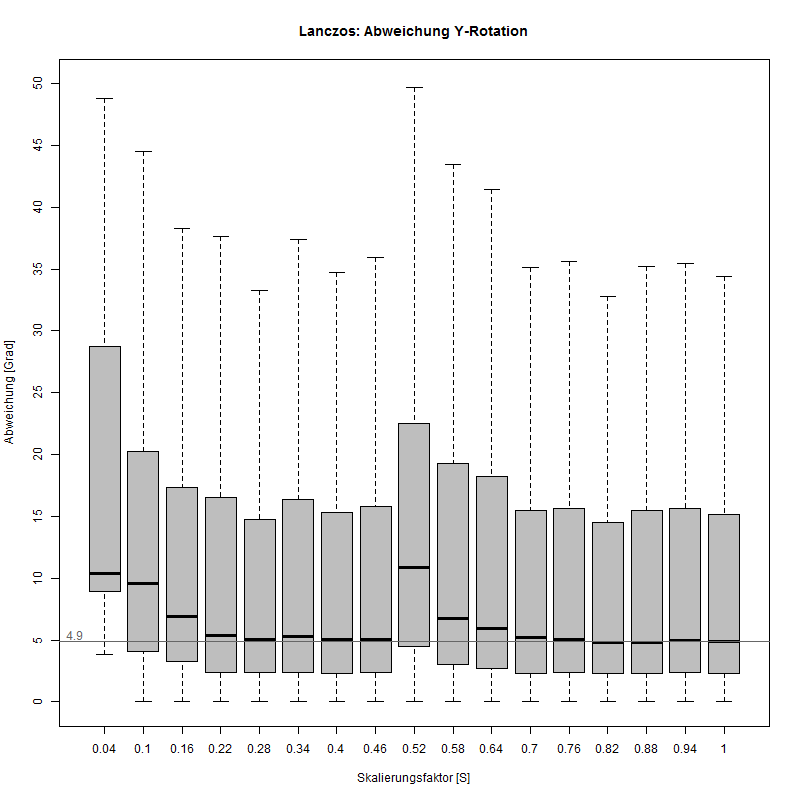
\includegraphics[width=0.245\linewidth]{img_Skalierung/LA_Ry}
	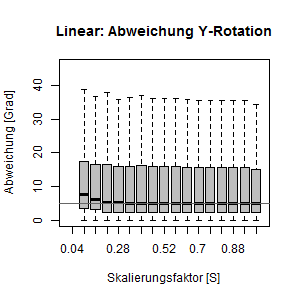
\includegraphics[width=0.245\linewidth]{img_Skalierung/LI_Ry}
	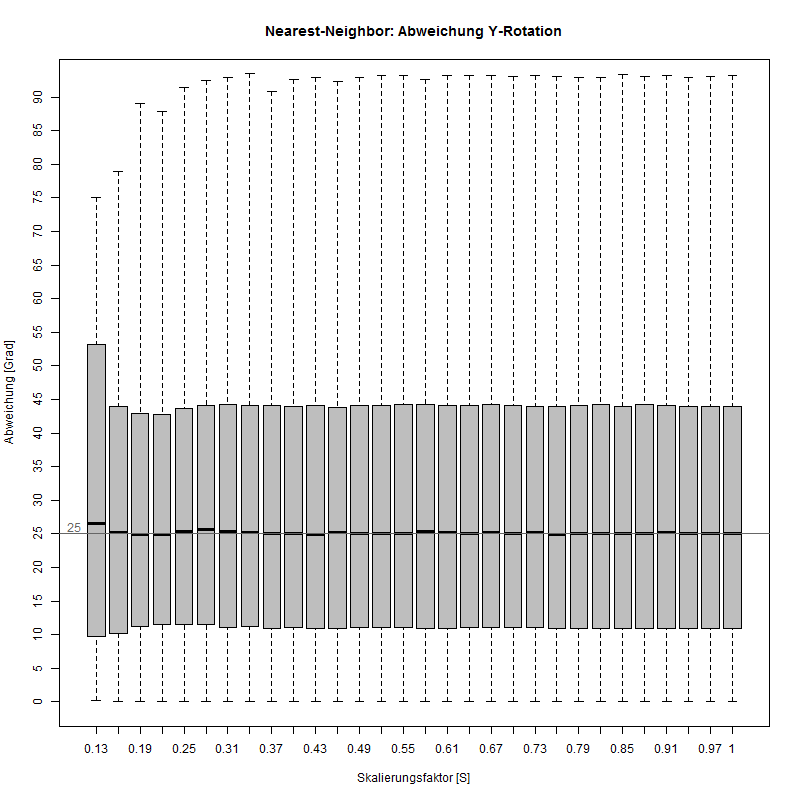
\includegraphics[width=0.245\linewidth]{img_Skalierung/NN_Ry}
	\caption{Zusammenhang zwischen der Skalierung (X-Achse) und der Abweichung des Winkels in X-Richtung, Angabe in Bogenmaß.\\
		Von rechts nach links: Bicubic, Lanczos, Linear, Nearest-Neighbor}
	\label{img_Y_Rot_Skal}
\end{figure}
\begin{figure}
	\centering
	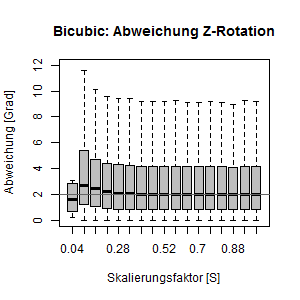
\includegraphics[width=0.245\linewidth]{img_Skalierung/CU_Rz}
	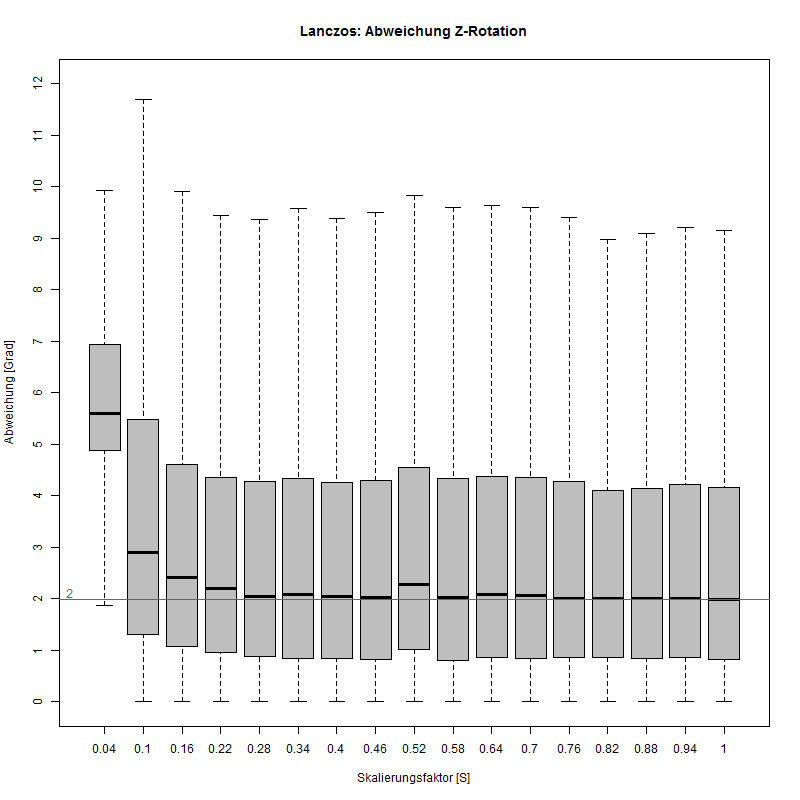
\includegraphics[width=0.245\linewidth]{img_Skalierung/LA_Rz}
	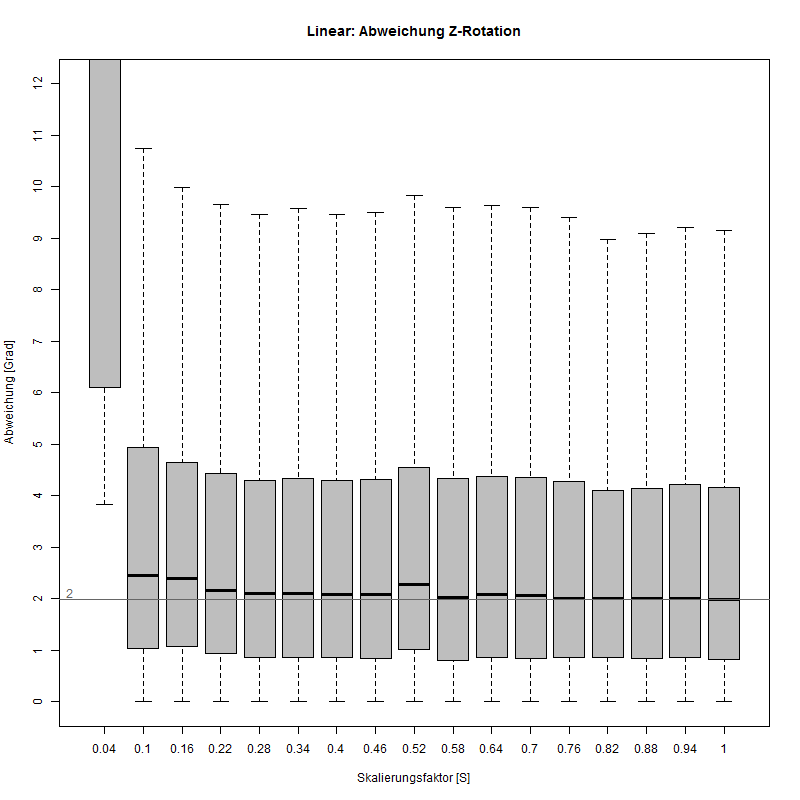
\includegraphics[width=0.245\linewidth]{img_Skalierung/LI_Rz}
	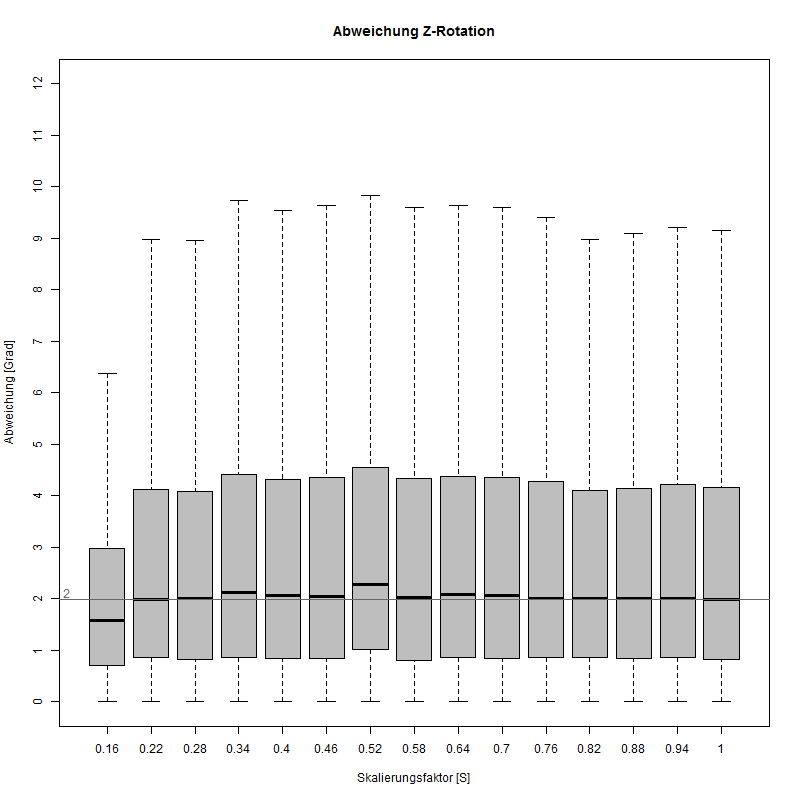
\includegraphics[width=0.245\linewidth]{img_Skalierung/NN_Rz}
	\caption{Zusammenhang zwischen der Skalierung (X-Achse) und der Abweichung des Winkels in Y-Richtung, Angabe in Bogenmaß.\\
		Von rechts nach links: Bicubic, Lanczos, Linear, Nearest-Neighbor}
	\label{img_Z_Rot_Skal}
\end{figure}
\begin{figure}
	\centering
	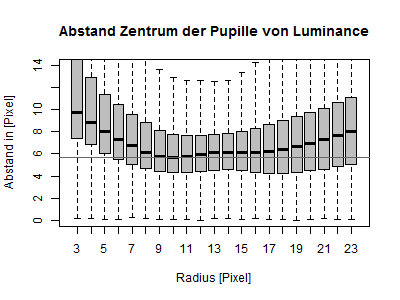
\includegraphics[width=0.32\linewidth]{Eye_Img_Box/Norm_Radius_A}
	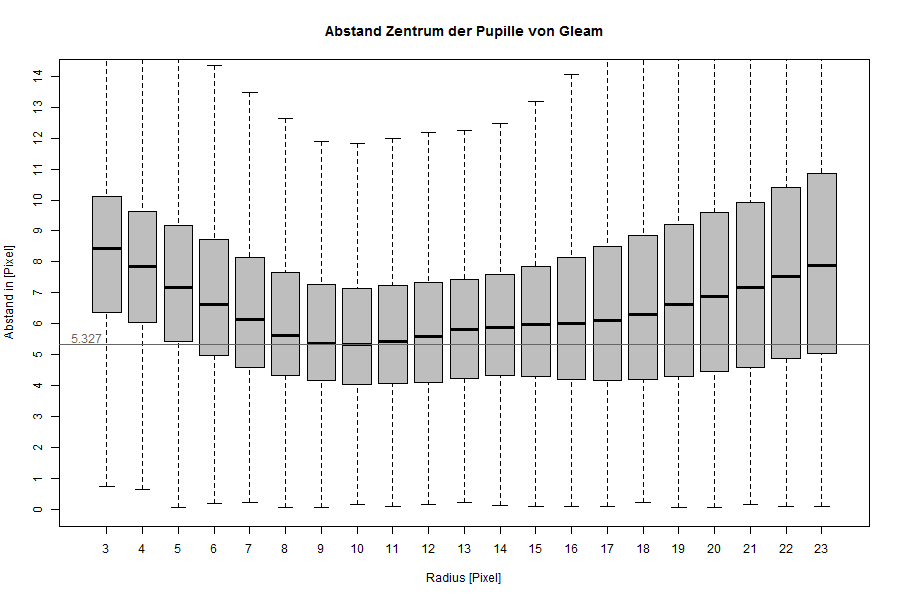
\includegraphics[width=0.32\linewidth]{Eye_Img_Box/Gleam_Radius_A}
	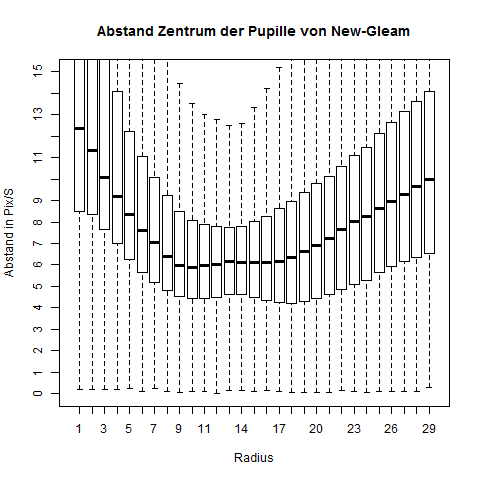
\includegraphics[width=0.32\linewidth]{Eye_Img_Box/New_Radius_A}\\
	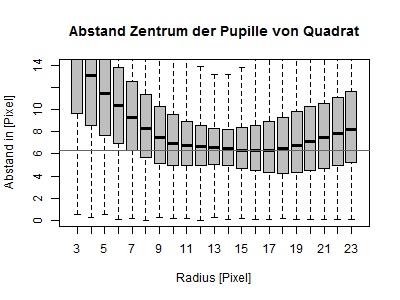
\includegraphics[width=0.32\linewidth]{Eye_Img_Box/Qua_Radius_A}
	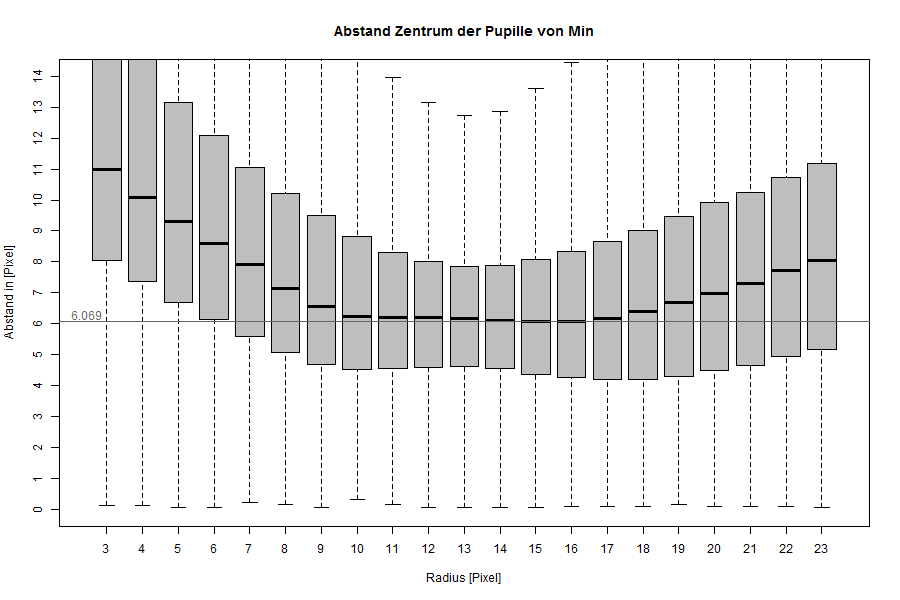
\includegraphics[width=0.32\linewidth]{Eye_Img_Box/Min_Radius_A}
	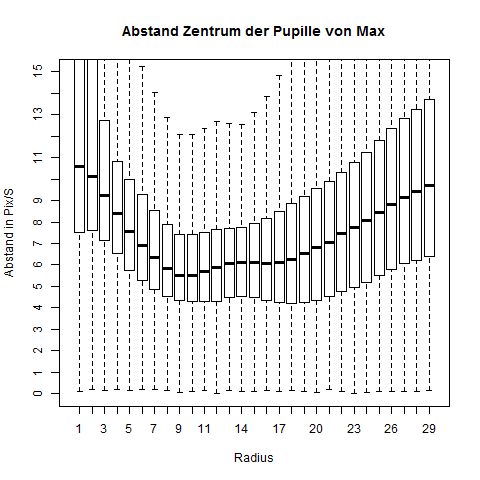
\includegraphics[width=0.32\linewidth]{Eye_Img_Box/Max_Radius_A}
	%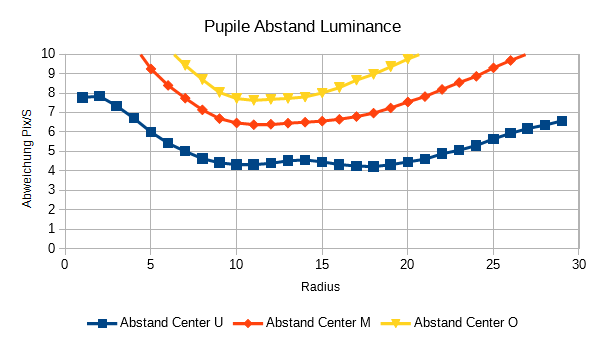
\includegraphics[width=0.49\linewidth]{Eye_Img/Normal_Abstand_P}
	%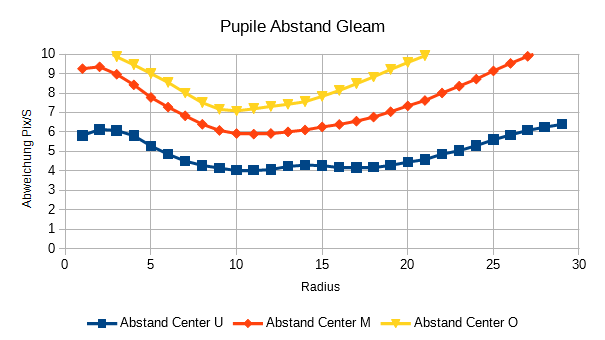
\includegraphics[width=0.49\linewidth]{Eye_Img/Gleam_Abstand_P}
	%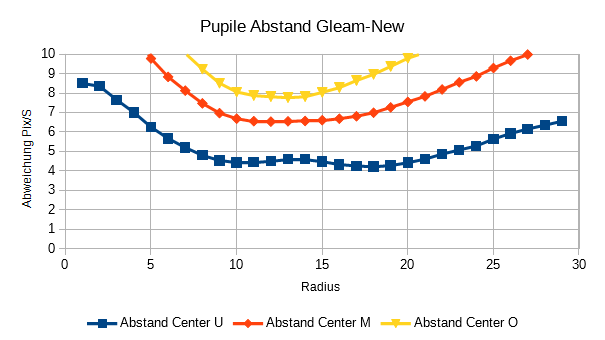
\includegraphics[width=0.49\linewidth]{Eye_Img/New_Abstand_P}
	%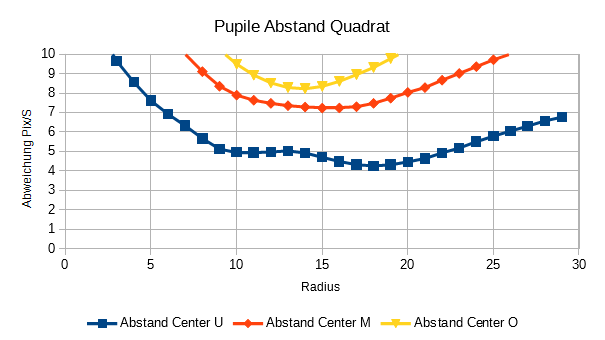
\includegraphics[width=0.49\linewidth]{Eye_Img/Quadrat_Abstand_P}
	%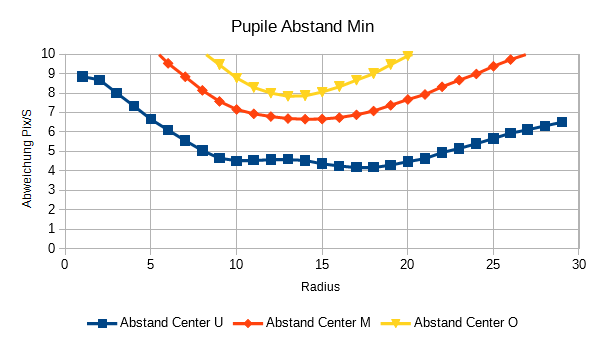
\includegraphics[width=0.49\linewidth]{Eye_Img/Min_Abstand_P}
	%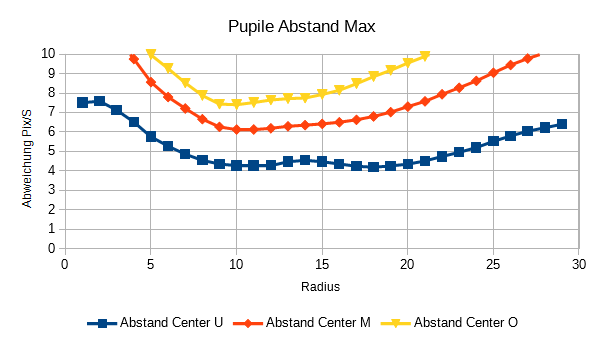
\includegraphics[width=0.49\linewidth]{Eye_Img/Max_Abstand_P}
	\caption{Abstand des Zentrums der Landmark-Pupille und der berechneten Ellipse in [Pixel] gegen den Radius-Größe des Filters.\\
		Oben-Links: Luminance, Oben-Mitte: Gleam, Oben-Rechts: Gleam New,\\ Unten-Links: Quadrat, Unten-Mitte: Min-Wert, Unten-Rechts: Max-Wert}
	\label{ElSe_Gray_Zentrum}
\end{figure}
\begin{figure}
	\centering
	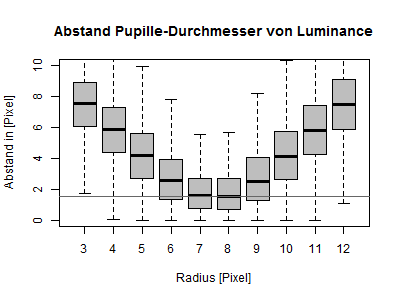
\includegraphics[width=0.32\linewidth]{Eye_Img_Box/Norm_Radius_P}
	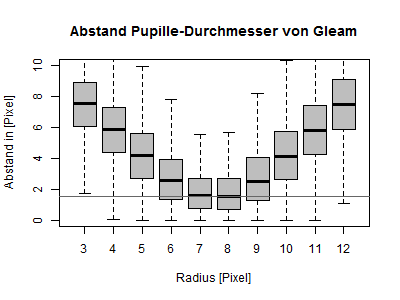
\includegraphics[width=0.32\linewidth]{Eye_Img_Box/Gleam_Radius_P}
	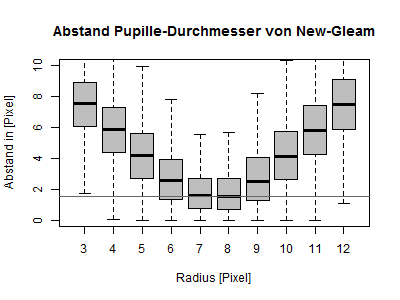
\includegraphics[width=0.32\linewidth]{Eye_Img_Box/New_Radius_P}\\
	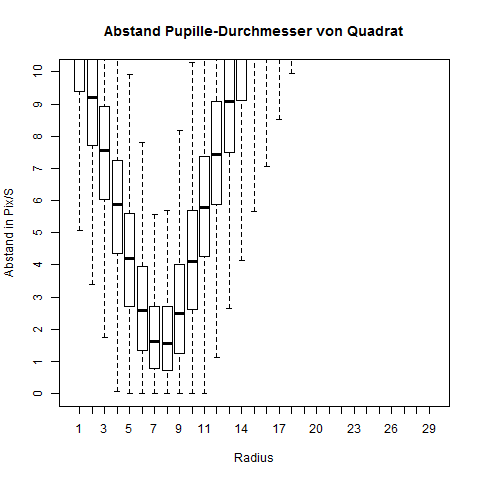
\includegraphics[width=0.32\linewidth]{Eye_Img_Box/Qua_Radius_P}
	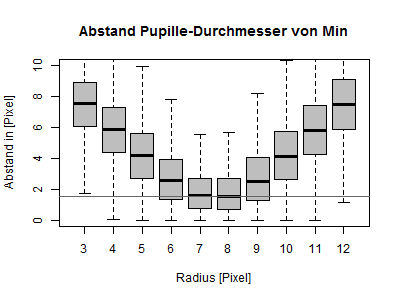
\includegraphics[width=0.32\linewidth]{Eye_Img_Box/Min_Radius_P}
	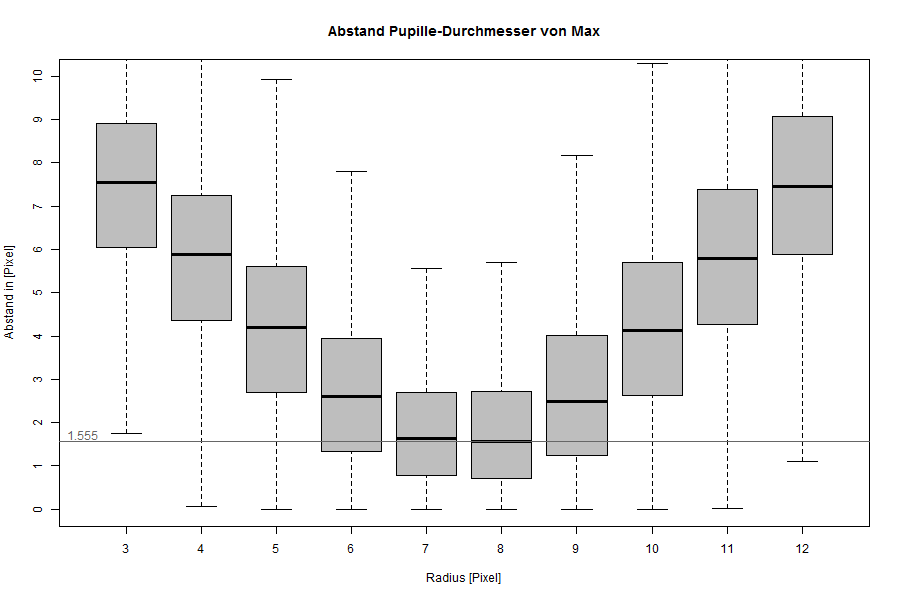
\includegraphics[width=0.32\linewidth]{Eye_Img_Box/Max_Radius_P}
	%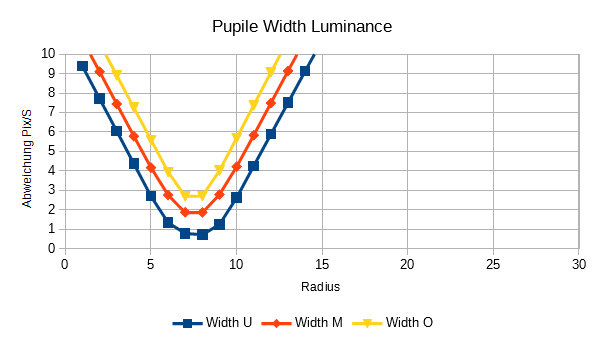
\includegraphics[width=0.49\linewidth]{Eye_Img/Normal_Width_P}
	%\includegraphics[width=0.49\linewidth]{Eye_Img/Gleam_Width_P}
	%\includegraphics[width=0.49\linewidth]{Eye_Img/New_Width_P}
	%\includegraphics[width=0.49\linewidth]{Eye_Img/Quadrat_Width_P}
	%\includegraphics[width=0.49\linewidth]{Eye_Img/Min_Width_P}
	%\includegraphics[width=0.49\linewidth]{Eye_Img/Max_Width_P}
	\caption{Unterschied Zwischen den Radien der Landmark-Pupille und der Berechneten Ellipse in [Pixel] gegen den Radius-Größe des Filters\\
		Oben-Links: Luminance, Oben-Mitte: Gleam, Oben-Rechts: Gleam New,\\ Unten-Links: Quadrat, Unten-Mitte: Min-Wert, Unten-Rechts: Max-Wert}
	\label{ElSe_Gray_Pupille}
\end{figure}
\begin{figure}
	\centering
	\includegraphics[width=0.32\linewidth]{Eye_Img_Box/Norm_Radius_I}
	\includegraphics[width=0.32\linewidth]{Eye_Img_Box/Gleam_Radius_I}
	\includegraphics[width=0.32\linewidth]{Eye_Img_Box/New_Radius_I}\\
	\includegraphics[width=0.32\linewidth]{Eye_Img_Box/Qua_Radius_I}
	\includegraphics[width=0.32\linewidth]{Eye_Img_Box/Min_Radius_I}
	\includegraphics[width=0.32\linewidth]{Eye_Img_Box/Max_Radius_I}
	%\includegraphics[width=0.49\linewidth]{Eye_Img/Normal_Width_I}
	%\includegraphics[width=0.49\linewidth]{Eye_Img/Gleam_Width_I}
	%\includegraphics[width=0.49\linewidth]{Eye_Img/New_Width_I}
	%\includegraphics[width=0.49\linewidth]{Eye_Img/Quadrat_Width_I}
	%\includegraphics[width=0.49\linewidth]{Eye_Img/Min_Width_I}
	%\includegraphics[width=0.49\linewidth]{Eye_Img/Max_Width_I}
	\caption{Unterschied Zwischen den Radien der Landmark-Iris und der Berechneten Ellipse in [Pixel] gegen den Radius-Größe des Filters.\\
		Oben-Links: Luminance, Oben-Mitte: Gleam, Oben-Rechts: Gleam New,\\ Unten-Links: Quadrat, Unten-Mitte: Min-Wert, Unten-Rechts: Max-Wert}
	\label{ElSe_Gray_Iris}
\end{figure}
\begin{figure}
	\centering
	\includegraphics[width=0.32\linewidth]{Eye_Img_Box/Gleam_Radius_P_8}
	\includegraphics[width=0.32\linewidth]{Eye_Img_Box/Norm_Radius_P_8}
	\includegraphics[width=0.32\linewidth]{Eye_Img_Box/Qua_Radius_P_8}\\
	\includegraphics[width=0.32\linewidth]{Eye_Img_Box/Gleam_Radius_A_10}
	\includegraphics[width=0.32\linewidth]{Eye_Img_Box/Norm_Radius_A_10}
	\includegraphics[width=0.32\linewidth]{Eye_Img_Box/Qua_Radius_A_16}\\
	\includegraphics[width=0.32\linewidth]{Eye_Img_Box/Gleam_Radius_I_18}
	\includegraphics[width=0.32\linewidth]{Eye_Img_Box/Norm_Radius_I_18}
	\includegraphics[width=0.32\linewidth]{Eye_Img_Box/Qua_Radius_I_18}
	\caption{Auswirkung von der Bildgröße auf die Qualität der Berechnung. Aufgetragen ist die Abweichung [Pixel/Skalierung] gegen den Skalierungsfaktor. Oben: Pupille-Durchmesser, Mitte Abweichung Zentrum, Iris-Durchmesser\\
		Links: Gleam, Mitte: Luminance, Rechts Quadrat}
	\label{ElSe_scall}
\end{figure}
\end{landscape}
\begin{figure}
	\centering
	\includegraphics[width=0.49\linewidth]{Eye_Img_Box/Openface_BoxX}
	\includegraphics[width=0.49\linewidth]{Eye_Img_Box/Openface_BoxY}\\
	\includegraphics[width=0.49\linewidth]{Eye_Img_Box/Openface_BoxW}
	\includegraphics[width=0.49\linewidth]{Eye_Img_Box/Openface_BoxH}
	%\includegraphics[width=0.245\linewidth]{Eye_Img/Box_X}
	%\includegraphics[width=0.245\linewidth]{Eye_Img/Box_Y}
	%\includegraphics[width=0.245\linewidth]{Eye_Img/Box_W}
	%\includegraphics[width=0.245\linewidth]{Eye_Img/Box_H}
	\caption{Bestimmung der Box ums Auge abhängig von der Bildgröße. Aufgetragen ist die Abweichung [Pixel/Skalierung] gegen den Skalierungsfaktor.\\
		Dargestellt sind Koordinaten, X- und Y-Position in Pixel sowie die Ausdehnung der Box (Width und Hight) ebenfalls in Pixel relativ zur umschließenden Box der Landmarks.}
	\label{OpenFace_Eye_Box}
\end{figure}
\begin{landscape}
	\begin{figure}
		\centering
		\includegraphics[width=0.192\linewidth]{OpenFace_Img/Head_x_Err_S1}
		\includegraphics[width=0.192\linewidth]{OpenFace_Img/Head_x_Err_S05}
		\includegraphics[width=0.192\linewidth]{OpenFace_Img/Head_x_Err_S025}
		\includegraphics[width=0.192\linewidth]{OpenFace_Img/Head_x_Err_S01}
		\includegraphics[width=0.192\linewidth]{OpenFace_Img/Head_x_Err_S005}\\	
		\includegraphics[width=0.192\linewidth]{OpenFace_Img/Head_y_Err_S1}
		\includegraphics[width=0.192\linewidth]{OpenFace_Img/Head_y_Err_S05}
		\includegraphics[width=0.192\linewidth]{OpenFace_Img/Head_y_Err_S025}
		\includegraphics[width=0.192\linewidth]{OpenFace_Img/Head_y_Err_S01}
		\includegraphics[width=0.192\linewidth]{OpenFace_Img/Head_y_Err_S005}\\	
		\includegraphics[width=0.192\linewidth]{OpenFace_Img/EyeAVG_x_Err_S1}	
		\includegraphics[width=0.192\linewidth]{OpenFace_Img/EyeAVG_x_Err_S05}
		\includegraphics[width=0.192\linewidth]{OpenFace_Img/EyeAVG_x_Err_S025}
		\includegraphics[width=0.192\linewidth]{OpenFace_Img/EyeAVG_x_Err_S01}
		\includegraphics[width=0.192\linewidth]{OpenFace_Img/EyeAVG_x_Err_S005}
		\caption{Abweichung der Videoaufnahme von der Kopfausrichtung Horizontal (Oben), Kopforientierung Vertikal (Mitte) und die X-Ausrichtung der Augen (Unten)\\Skalierungsfaktor von links nach rechts (1/0.5/0.25/0.1/0.05), Y-Achse: $[0-35]^\circ$}
		\label{graph_VideoSkalierung_Err}
	\end{figure}
\end{landscape}
